\documentclass[a4paper,11pt]{article}
\usepackage[svgnames, dvipsnames, table]{xcolor}
\usepackage{WriteOnGrid}
\usepackage{amsmath,amssymb}
\usepackage{lipsum}
\definecolor{myblue}{HTML}{0039a6}
\setlength{\jot}{.44cm}

\newcommand*\circled[1]{%
	\tikz[baseline=(char.base)]{%
		\node[shape=circle, draw, inner sep=1pt] (char) {#1};
	}%
}

\begin{document}
\pagestyle{empty}
\begin{PleinePageCinqCinq}[CouleurMarge=lightgray!50]
	\xdef\CCFullMargeG{3.7}
	\xdef\CCFullMargeH{1.3}
	\draw[red!75,thick]
	($(current page.north west)+(\CCFullMargeG,0)$) --
	($(current page.south west)+(\CCFullMargeG,0)$) ;
	\coordinate (CinqCinqOrigine) at
	($(current page.north west)+({\CCFullMargeG},{-\CCFullMargeH})$) ;

	\xdef\CCFullLargPap{24.7}
	\renewcommand\CadreNoteCinqCinq[2][3]{%on précise la {ligne de début} + [hauteur]
		%cadre de note
		\draw[thick, red]
		($(current page.north west)+(0,{(-#2+1)*0.5-\CCFullMargeH})$) --++
		({\CCFullLargPap-\CCFullMargeG},{0}) ;
		\draw[thick, red]
		($(current page.north west)+(0,{(-#2+1-#1)*0.5-\CCFullMargeH})$) --++
		({\CCFullLargPap-\CCFullMargeG},{0}) ;
		\draw[thick, red]
		($(current page.north west)+(0,{(-#2+1-#1)*0.5-\CCFullMargeH})$) --++
		({#1.*0.5+.2},{#1*0.5}) ;
	}
	\LignePapierCinqCinq[Echelle=1.25,Ligne=1,Largeur=17,Couleur=myblue]{%
		\hspace{-2.5cm}NICOLAS}
	\LignePapierCinqCinq[Echelle=1.25,Ligne=1,Largeur=17,Couleur=myblue]<center>{%
		\hspace{-1cm}{\Large DS 1 de Physique-Chimie}}
	\LignePapierCinqCinq[Echelle=1.25,Ligne=3,Largeur=17,Couleur=myblue]<center>{%
		\hspace{-1cm}{\Large Optique géométrique}}
	\LignePapierCinqCinq[Echelle=1.25,Ligne=2,Largeur=17,Couleur=myblue]<right>{%
		Le 27/09/24}
	\LignePapierCinqCinq[Echelle=1.25,Ligne=2,Largeur=17,Couleur=myblue]{%
		\hspace{-2.5cm}Nora}
	\LignePapierCinqCinq[Echelle=1.25,Ligne=3,Largeur=17,Couleur=myblue]{%
		\hspace{-2.5cm}MPSI3}
	% \LignePapierCinqCinq[Echelle=1.25,Ligne=3,Couleur=red]<center>{\underline{\bfseries Devoir 2}}
	\CadreNoteCinqCinq[7]{5}
	\coordinate (CinqCinqOrigine) at
	($(current page.north west)+({\CCFullMargeG+0.5},{-\CCFullMargeH})$) ;
	\ParagraphePapierCinqCinq[Ligne=14,Largeur=17,Couleur=myblue]{%
		\underline{\Large Remarques antérieures}
		\\
		$\diamond$ Les lentilles divergentes n’ont rien de spécial~!
		\\
		$\diamond$ Conditions de Gauss mal comprises, confondues avec leurs
		conséquences (stigmatisme,\\ aplanétisme).
		\\[-.5cm]\hspace*{-0.52cm}\rule{\linewidth}{0.4pt}}
	\ParagraphePapierCinqCinq[Ligne=23,Couleur=myblue]{%
		\underline{\Large Remarques personnelles}
		\\\\\\\\\\\hspace*{-0.52cm}\rule{\linewidth}{0.4pt}}
	\LignePapierCinqCinq[Ligne=35,Largeur=17,Couleur=myblue]{%
		\underline{\Large E1) Étude de quelques lentilles minces}}
	\ParagraphePapierCinqCinq[Ligne=37,Largeur=17,Couleur=myblue]{%
		A) \circled{1}
		\smallbreak
		\noindent
		\begin{minipage}[c]{.48\linewidth}
			\vspace{.27cm}
			\hspace{-.15cm}
			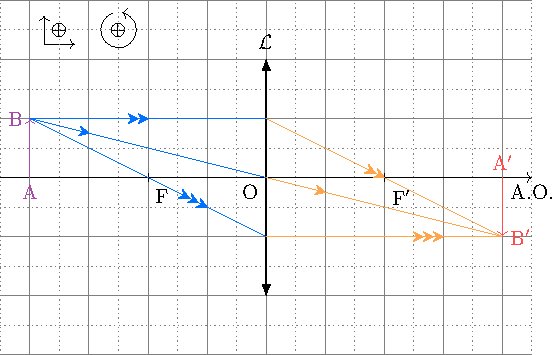
\includegraphics[scale=1]{./figures/E1/convAF}
		\end{minipage}
		\hfill
		\begin{minipage}[c]{.42\linewidth}
			On obtient donc une image \underline{réelle},
			\smallbreak
			\underline{renversée} et de \underline{même taille} que
			\smallbreak
			l'objet.
			\smallbreak
			Avec la relation de \textsc{Descartes}~:
		\end{minipage}
	}
	\LignePapierCinqCinq[Ligne=52,Largeur=17,Couleur=myblue]{%
		\circled{2} …}
	\draw[thick, myblue]
	($(current page.south east)+(-1.8,0)$)
	coordinate (BRL) --++
	(0,1.4)
	coordinate (BRC) --++
	(1.8,0)
	coordinate (BRR)
	%
	(BRL) -- (BRR);
	\coordinate (BR) at (current page.south east);
	\node[myblue, scale=2] at (barycentric cs:BRL=1,BRC=1,BRR=1) {$1$};
	\node[myblue, scale=2] at (barycentric cs:BR=1,BRL=1,BRR=1) {$2$};
\end{PleinePageCinqCinq}

\clearpage
\pagestyle{empty}
\begin{PleinePageCinqCinq}[CouleurMarge=lightgray!50]
	\draw[red!75,thick]
	($(current page.north west)+(\CCFullMargeG,0)$) --
	($(current page.south west)+(\CCFullMargeG,0)$) ;
	\coordinate (CinqCinqOrigine) at
	($(current page.north west)+({\CCFullMargeG},{-\CCFullMargeH})$) ;
\end{PleinePageCinqCinq}

\clearpage
\pagestyle{empty}
\begin{PleinePageCinqCinq}[CouleurMarge=lightgray!50]
	\draw[red!75,thick]
	($(current page.north west)+(\CCFullMargeG,0)$) --
	($(current page.south west)+(\CCFullMargeG,0)$) ;
	\coordinate (CinqCinqOrigine) at
	($(current page.north west)+({\CCFullMargeG},{-\CCFullMargeH})$) ;
\end{PleinePageCinqCinq}

\clearpage
\pagestyle{empty}
\begin{PleinePageCinqCinq}[CouleurMarge=lightgray!50]
	\draw[red!75,thick]
	($(current page.north west)+(\CCFullMargeG,0)$) --
	($(current page.south west)+(\CCFullMargeG,0)$) ;
	\coordinate (CinqCinqOrigine) at
	($(current page.north west)+({\CCFullMargeG},{-\CCFullMargeH})$) ;
\end{PleinePageCinqCinq}

\clearpage
\pagestyle{empty}
\begin{PleinePageCinqCinq}[CouleurMarge=lightgray!50]
	\draw[red!75,thick]
	($(current page.north west)+(\CCFullMargeG,0)$) --
	($(current page.south west)+(\CCFullMargeG,0)$) ;
	\coordinate (CinqCinqOrigine) at
	($(current page.north west)+({\CCFullMargeG},{-\CCFullMargeH})$) ;

	\LignePapierCinqCinq[Echelle=1.25,Ligne=1,Largeur=17,Couleur=myblue]{%
		\hspace{-2.5cm}NICOLAS}
	\LignePapierCinqCinq[Echelle=1.25,Ligne=1,Largeur=17,Couleur=myblue]<center>{%
		\hspace{-1cm}{\Large DS 1 -- Suite}}
	\LignePapierCinqCinq[Echelle=1.25,Ligne=2,Largeur=17,Couleur=myblue]{%
		\hspace{-2.5cm}Nora}
	\LignePapierCinqCinq[Echelle=1.25,Ligne=3,Largeur=17,Couleur=myblue]{%
		\hspace{-2.5cm}MPSI3}
	\draw[thick, myblue]
	($(current page.south east)+(-1.8,0)$)
	coordinate (BRL) --++
	(0,1.4)
	coordinate (BRC) --++
	(1.8,0)
	coordinate (BRR)
	%
	(BRL) -- (BRR);
	\coordinate (BR) at (current page.south east);
	\node[myblue, scale=2] at (barycentric cs:BRL=1,BRC=1,BRR=1) {$2$};
	\node[myblue, scale=2] at (barycentric cs:BR=1,BRL=1,BRR=1) {$2$};
\end{PleinePageCinqCinq}

\clearpage
\pagestyle{empty}
\begin{PleinePageCinqCinq}[CouleurMarge=lightgray!50]
	\draw[red!75,thick]
	($(current page.north west)+(\CCFullMargeG,0)$) --
	($(current page.south west)+(\CCFullMargeG,0)$) ;
	\coordinate (CinqCinqOrigine) at
	($(current page.north west)+({\CCFullMargeG},{-\CCFullMargeH})$) ;
\end{PleinePageCinqCinq}

\clearpage
\pagestyle{empty}
\begin{PleinePageCinqCinq}[CouleurMarge=lightgray!50]
	\draw[red!75,thick]
	($(current page.north west)+(\CCFullMargeG,0)$) --
	($(current page.south west)+(\CCFullMargeG,0)$) ;
	\coordinate (CinqCinqOrigine) at
	($(current page.north west)+({\CCFullMargeG},{-\CCFullMargeH})$) ;
\end{PleinePageCinqCinq}

\clearpage
\pagestyle{empty}
\begin{PleinePageCinqCinq}[CouleurMarge=lightgray!50]
	\draw[red!75,thick]
	($(current page.north west)+(\CCFullMargeG,0)$) --
	($(current page.south west)+(\CCFullMargeG,0)$) ;
	\coordinate (CinqCinqOrigine) at
	($(current page.north west)+({\CCFullMargeG},{-\CCFullMargeH})$) ;
\end{PleinePageCinqCinq}

\end{document}
